% \mychapter{3}{Testing}
\mychapter{4}{Results}

Using the previously derived stability criterion, the affect that the different stabilisation types have on the backflow for different parameter values can be tested, and if they are able to attain the stability criterion. The first case that will be looked into is the case where there is no added stability term and checking whether indeed the unstabilised backflow is causing there to be negative eigenvalues once discretised. Following this, the effect of the different stabilisations will be observed on the eigenvalues to see how easily they can be automated, which will provide the necessary information needed in the next chapter where, if possible, the algorithms will be presented for the automation of the different backflow stabilisation method parameters.

\section{Testing environment}

In order to conduct the investigations, the FEniCS package\footnote{\url{https://fenicsproject.org/}} for the Python programming language will be used in conjunction with a relatively general test case. The tests will be performed on a specific geometry, a representation of a tubular organ(vein, wind pipe, etc.) with a stenosis, which is a commonly occurring physiological problem, and thus a geometry which could often be encountered when solving the problems. The geometry will look as follows:\\
\begin{figure}[h]
\centering

\includegraphics[width=0.5\textwidth]{latex/Thesis/media/stenosis.png}
\caption{The geometry on which the tests will be performed\label{fig:testgeo}}
\end{figure}

where the specific weak form being solved is (in FEmiCS notation):
\begin{align*}
    F = &k\rho\inner{\bmu - \bmu 0}{\bmv}_{\Omega} + \mu\inner{\nabla\bmu_-}{\nabla\bmv}_{\Omega} -\\ &\inner{p_-}{\nabla\cdot\bmv}_{\Omega} + \inner{q}{\nabla\cdot\bmu}_{\Omega} +\\ &\rho\inner{\qty(\nabla\bmu_-)\bmu}{\bmv}_{\Omega} + \frac{\rho}{2}\inner{\nabla\cdot\bmu 0}{\bmu_-\cdot\bmv}_{\Omega} + S
\end{align*}
where \mathm{S=\qty{S_{Vel}, S_{TangMax}, S_{Tang}}}, \mathm{\mu = 0.035}, \mathm{\rho = 1.2} and \mathm{k = \frac{1}{\text{d}t}} with d\mathm{t} the chosen time step. A relatively high Reynolds number of 5000 is used as backflow effects are stronger with higher Reynolds numbers. The top boundary is specified with a no-slip condition and the bottom boundary has a free-slip and no-penetration condition. The inflow term coming from the left boundary is (in FEmiCS notation):
\[
    \bmu(t)~=~\sin\qty(at\pi)*U*(1 - pow(\bm{x}[1], 2))
\]
where \mathm{\bm{x} = [x~~y]}. The right boundary is the before mentioned homogeneous natural boundary condition which is satisfied once a solution has been found.

\section{Effect of different stabilisations}
Now the effect the different stabilisations have on the eigenvalues of \mathm{-B+S} will be observed. So first a time step in the simulation is selected where backflow is occurring, and then it will observed what effect changing the parameters of our stabilisation methods has on the eigenvalues.

\subsection{No Stabilisation}
One of the first tests that would be important to conduct is to verify that our stability criterion is not attained in the presence of backflow with no stabilisation added. Thus just the eigenvalues of the discretisation of \mathm{- B} as defined in \autoref{eq:backflow} will be observed. What is expect is that there are a few negative eigenvalues which would be responsible for the instabilities seen during the simulation and indeed in \autoref{fig:Nostabmulti} one sees that it is indeed the case that there are negative eigenvalues for various times when there is backflow occurring. An interesting observation to note is that the eigenvalues change for each times step, which would make it nearly impossible to find a stable value for the parameters before the simulation except for the theoretically stable values.

\begin{figure}[ht]
     \centering
     \begin{subfigure}[h]{0.3\textwidth}
        \centering
        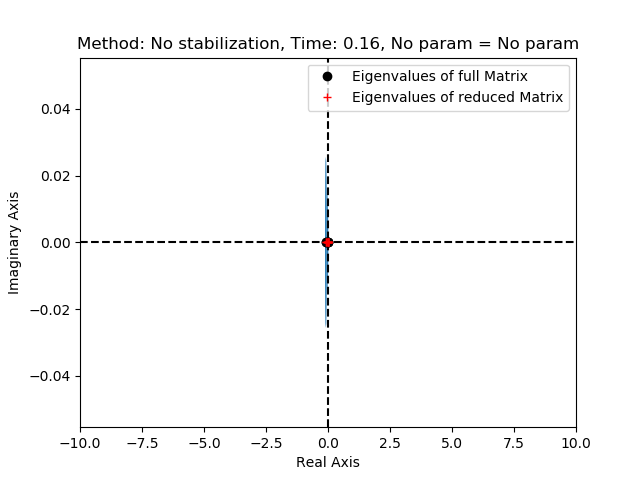
\includegraphics[width=\textwidth]{latex/Thesis/media/NoStab1.png}
        % \caption{Minimum and maximum eigenvalues\label{fig:VeloEig}}
     \end{subfigure}
     \hfill
     \begin{subfigure}[h]{0.3\textwidth}
        \centering
        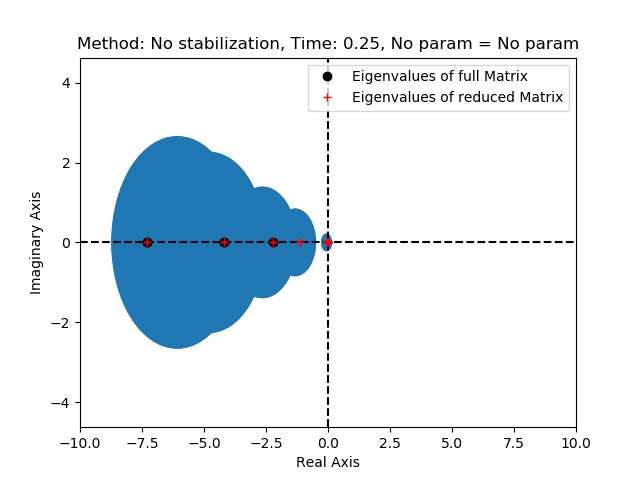
\includegraphics[width=\textwidth]{latex/Thesis/media/NoStab2.png}
        % \caption{Minimum eigenvalues\label{fig:VeloEigMin}}
     \end{subfigure}
     \hfill
     \begin{subfigure}[h]{0.3\textwidth}
        \centering
        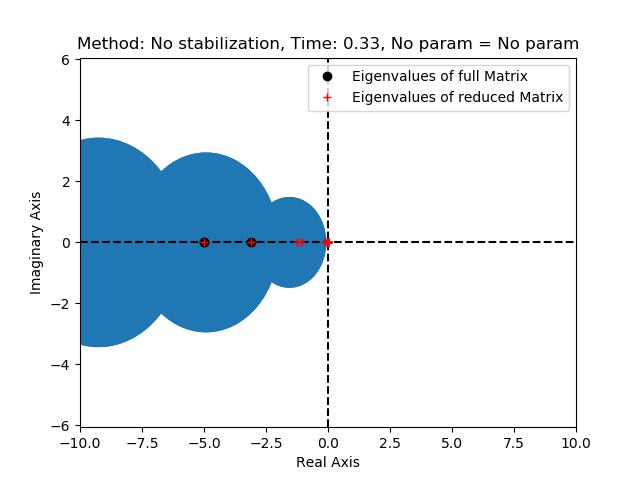
\includegraphics[width=\textwidth]{latex/Thesis/media/NoStab3.png}
        % \caption{Minimum eigenvalues\label{fig:VeloEigMin}}
     \end{subfigure}
        \caption{Eigenvalues for no stabilisation at different time steps}
        \label{fig:Nostabmulti}
\end{figure}

\includecomment{Include there a picture of the eigenvalues becoming negative with no stabilisation}

\includecomment{Also note something about how the flow changes at every time step so cannot select a single parameter before computation, besides 1, that guarantees stability}

\subsection{Velocity Penalisation}
The first stabilisation method which will be considered is the Velocity Penalisation method as defined in \autoref{eq:stabVeloPen}, and as noted before, this method has been proven to guarantee stability for a parameter value \mathm{\beta = 1}, so it would be expected that there would not be a negative eigenvalue for that value of \mbeta. First consider \autoref{fig:VeloEig} where the maximum and minimum eigenvalues of the discretisation of \mathm{-B + S} are plotted, as well as the difference between those extremum eigenvalues.
\begin{figure}[ht]
     \centering
     \begin{subfigure}[h]{0.49\textwidth}
        \centering
        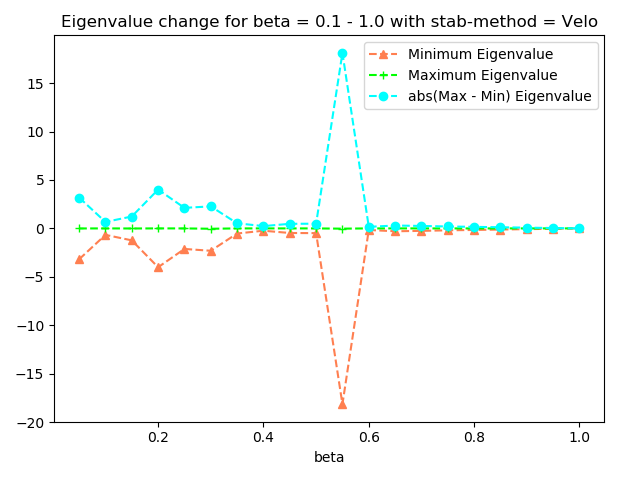
\includegraphics[width=\textwidth]{latex/Thesis/media/Beta_1_thru_0_velo.png}
        \caption{Minimum and maximum eigenvalues\label{fig:VeloEig}}
     \end{subfigure}
     \hfill
     \begin{subfigure}[h]{0.49\textwidth}
        \centering
        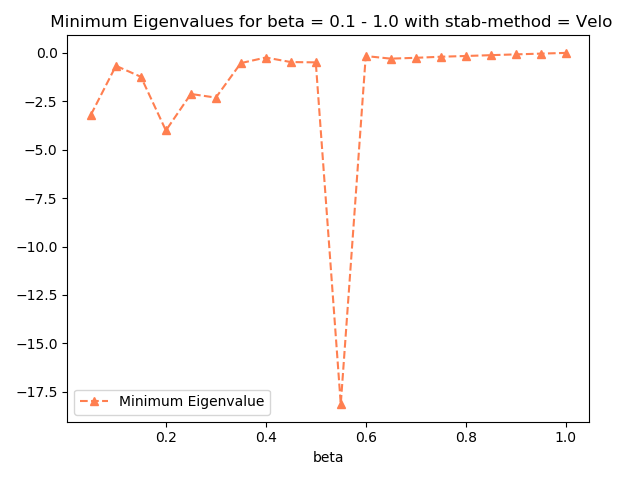
\includegraphics[width=\textwidth]{latex/Thesis/media/Beta_1_thru_0_velo_min.png}
        \caption{Minimum eigenvalues\label{fig:VeloEigMin}}
     \end{subfigure}
        \caption{Eigenvalues when using the Velocity Penalisation Stabilisation for various \mbeta's}
        \label{fig:VeloEigmulti}
\end{figure}
What can first be noted from \autoref{fig:VeloEig} is that when \mbeta~is less than one, the minimum eigenvalue appears to become negative. To see this in greater detail one can look to \autoref{fig:VeloEigMin} where only the minimum eigenvalue is plotted as a function of \mbeta. This Figure more clearly shows that if \mbeta~is decreased lower than one, then it may be possible for there to be a negative eigenvalue. This presents quite a problem for a basic automation process since it means that if values for \mbeta~lower than 1 are to be considered, then other terms would need to be considered which also help counteract the backflow instabilities. However, this would also increase the computational cost of the automation as in general these extra terms are much more computationally expensive to compute, and would significantly slow down the automation if they need to be calculated multiple times per time step.

\subsection{Tangential Penalisation Max}
The second stabilisation method to be considered is the Tangential Penalisation Max method as defined in \autoref{eq:stabTangPenMax} which has also been analytically proven to have a value of \mgamma~where stability is guaranteed. Thus it would be expected that if \mgamma~is sufficiently large, negative eigenvalues would no longer be observed and thus stability would be attained. First look to \autoref{fig:TangMaxEigLow} where as before the maximum and minimum eigenvalues of \mathm{-B+S} has been plotted and also to \autoref{fig:TangMaxEigLowMin} where only the minimum eigenvalue has been plotted as a function of \mgamma. From this range of \mgamma's, no conclusive statement can be made about whether the eigenvalues are now all becoming positive, so thus consider \autoref{fig:TangMaxEigHigh} and \autoref{fig:TangMaxEigHighMin} where a much larger range of \mgamma's is shown and now its clearly seen that the minimum eigenvalue is being made positive if gamma is made large enough. Thus, just by using the stabilising term of the Tangential Penalisation Max Method, the conditions of the stability criterion are satisfied without relying on any other terms to aid with combating the backflow.
\begin{figure}[ht]
     \centering
     \begin{subfigure}[h]{0.49\textwidth}
        \centering
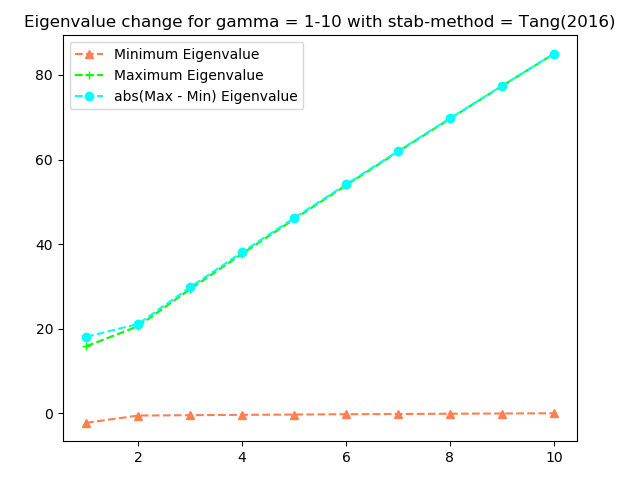
\includegraphics[width=\textwidth]{latex/Thesis/media/Gamma_1_thru_10_tang(2016).png}
\caption{Minimum and maximum eigenvalues\label{fig:TangMaxEigLow}}
     \end{subfigure}
     \hfill
     \begin{subfigure}[h]{0.49\textwidth}
\centering
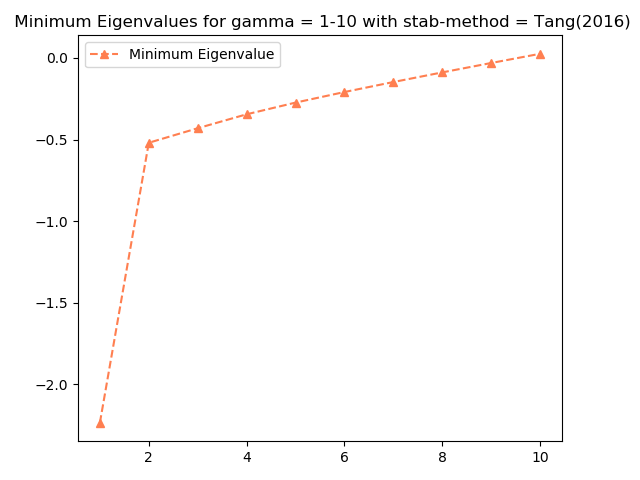
\includegraphics[width=\textwidth]{latex/Thesis/media/Gamma_1_thru_10_tang(2016)_min.png}
\caption{Minimum eigenvalues\label{fig:TangMaxEigLowMin}}
     \end{subfigure}
        \caption{Eigenvalues when using the Tangential Penalisation Max Stabilisation for \mgamma~ranging from 1 through 10}
        \label{fig:TangMaxEigLowmulti}
\end{figure}
\begin{figure}[ht]
     \centering
     \begin{subfigure}[h]{0.49\textwidth}
        \centering
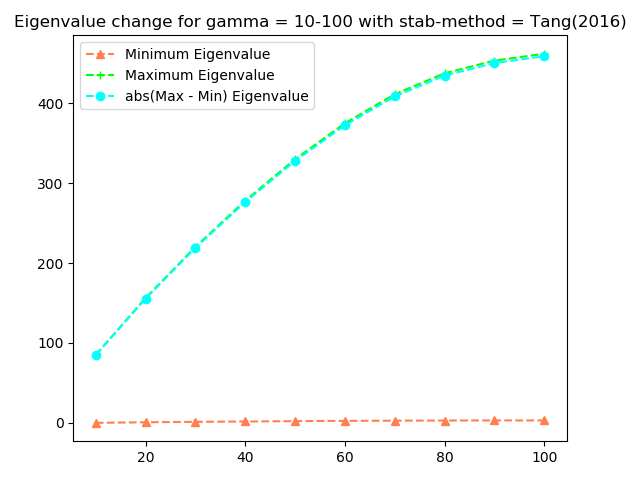
\includegraphics[width=\textwidth]{latex/Thesis/media/Gamma_10_thru_100_tang(2016).png}
\caption{Minimum and maximum eigenvalues\label{fig:TangMaxEigHigh}}
     \end{subfigure}
     \hfill
     \begin{subfigure}[h]{0.49\textwidth}
\centering
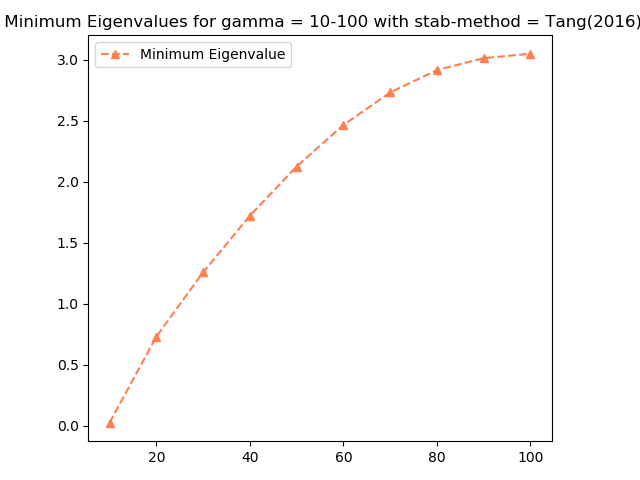
\includegraphics[width=\textwidth]{latex/Thesis/media/Gamma_10_thru_100_tang(2016)_min.png}
\caption{Minimum eigenvalues\label{fig:TangMaxEigHighMin}}
     \end{subfigure}
        \caption{Eigenvalues when using the Tangential Penalisation Max Stabilisation for \mgamma~ranging from 10 through 100}
        \label{fig:TangMaxEigHighmulti}
\end{figure}



\subsection{Tangential Penalisation}

The final stabilisation method to be considered is the Tangential Penalisation method as defined in \autoref{eq:stabTangPen} which has not been proven to have a value of \mgamma~such that stability is guaranteed, so it would greatly benefit from automation. From \autoref{fig:TangEigLowmulti} it would appear to have similar behaviour to that of \autoref{fig:TangMaxEigLowmulti} however no conclusive findings can be found. It is when going to \autoref{fig:TangEigHighmulti} that the problem becomes evident. No matter how large \mgamma~is taken, the minimum eigenvalue is unable to be pushed positive, rather it always remains negative. This requires further investigation as to why there is always a single eigenvalue that will not be made positive and if there are methods that could be employed that might solve this issue, such as employing pole placement.
\begin{figure}[ht]
     \centering
     \begin{subfigure}[h]{0.49\textwidth}
        \centering
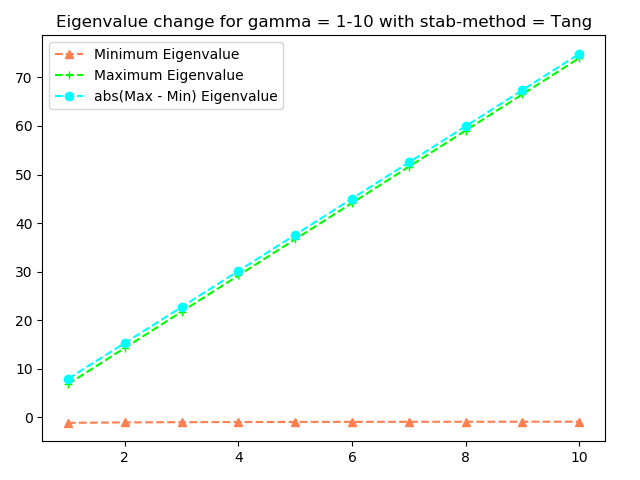
\includegraphics[width=\textwidth]{latex/Thesis/media/Gamma_1_thru_10_tang.png}
\caption{Minimum and maximum eigenvalues\label{fig:TangEigLow}}
     \end{subfigure}
     \hfill
     \begin{subfigure}[h]{0.49\textwidth}
\centering
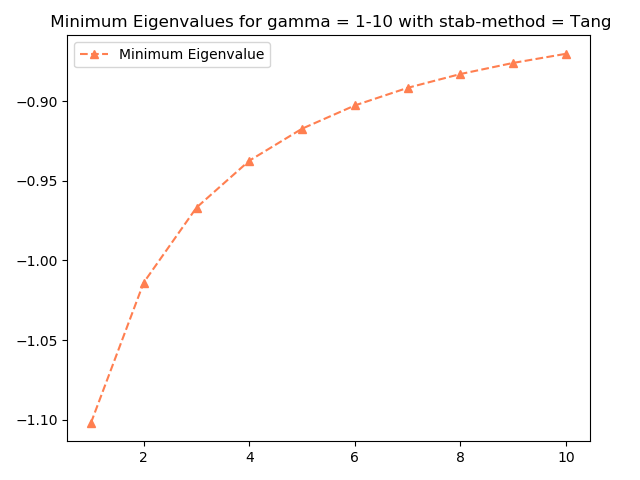
\includegraphics[width=\textwidth]{latex/Thesis/media/Gamma_1_thru_10_tang_min.png}
\caption{Minimum eigenvalues\label{fig:TangEigLowMin}}
     \end{subfigure}
        \caption{Eigenvalues when using the Tangential Penalisation Stabilisation for \mgamma~ranging from 1 through 10}
        \label{fig:TangEigLowmulti}
\end{figure}
\begin{figure}[ht]
     \centering
     \begin{subfigure}[h]{0.49\textwidth}
        \centering
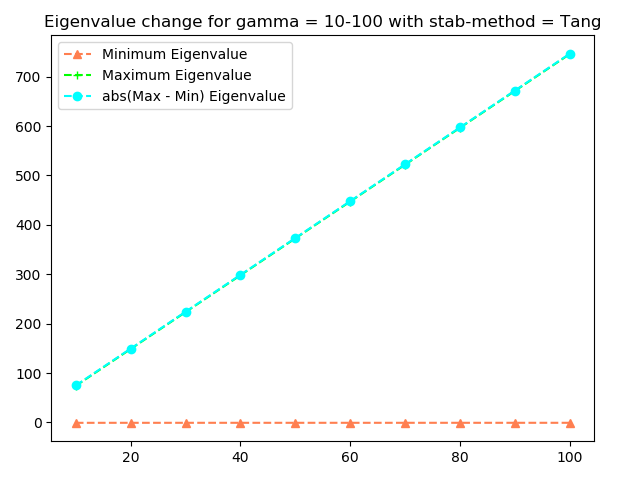
\includegraphics[width=\textwidth]{latex/Thesis/media/Gamma_10_thru_100_tang.png}
\caption{Minimum and maximum eigenvalues\label{fig:TangEigHigh}}
     \end{subfigure}
     \hfill
     \begin{subfigure}[h]{0.49\textwidth}
\centering
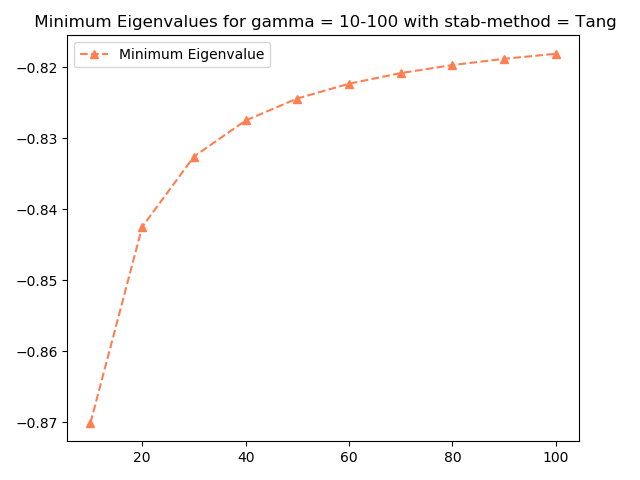
\includegraphics[width=\textwidth]{latex/Thesis/media/Gamma_10_thru_100_tang_min.png}
\caption{Minimum eigenvalues\label{fig:TangEigHighMin}}
     \end{subfigure}
        \caption{Eigenvalues when using the Tangential Penalisation Stabilisation for \mgamma~ranging from 10 through 100}
        \label{fig:TangEigHighmulti}
\end{figure}